\documentclass[a4paper,10pt]{article}

\usepackage[utf8]{inputenc}
\usepackage[T1]{fontenc}
\usepackage[english]{babel}

\usepackage{color}
\usepackage{float}
\usepackage{fancyvrb}

\usepackage{amssymb}
\usepackage{amsmath}
\usepackage{listings}
\usepackage{comment} 

\usepackage{graphicx}
\DeclareGraphicsExtensions{.png}

\definecolor{dkgreen}{rgb}{0,0.45,0}
\definecolor{gray}{rgb}{0.5,0.5,0.5}
\definecolor{mauve}{rgb}{0.30,0,0.30}

% Default settings for code listings
% Default settings for code listings
\lstset{frame=tb,
  language=Java,
  aboveskip=3mm,
  belowskip=3mm,
  showstringspaces=false,
  columns=flexible,
  basicstyle={\small\ttfamily},
  numbers=left,
  numberstyle=\footnotesize,
  keywordstyle=\color{dkgreen}\bfseries,
  commentstyle=\color{dkgreen},
  stringstyle=\color{mauve},
  frame=single,
  breaklines=true,
  breakatwhitespace=false
  tabsize=1
}

%indsætjeres navn herunder.
\title{Database-programming project
\\\rule{10cm}{0.5mm}}
\author{Andreas Toftegaard
\\Supervisor: Jan Baumbach \& Anders Moeslund\\ DM505\\\rule{5.5cm}{0.5mm}\\}
\date{April 6th 2016}

\begin{document}

\maketitle

\vfill

\tableofcontents
%laver forside og indholsfortegnelse

\newpage
\section{Specification} 
%forklar hvad programmet skal gøre
This assignment called for the design and implementation of a database to be used in a computer-store, managing all products for sale. The database would have means of approach, in the form of a java-application, to be able to view the contents of the database. Together, the application and database should be able to perform several operations defined in the assignment (project.pdf). 
\section{Design}
%hvordan projektet blev planlagt, hvilke tanker gik ind i hvordan problemet skulle løses
From the beginning, I adopted the idea of programming functionalities into the application in chronological order, as they were listed in the assignment. The database itself was the obvious starting point, as it was on this that the application would extract data. The database would ensure some constraints on the various products in the system, though I implemented some of these in the java-application and some by constructing the database-data appropriately. On top of this, the application would be placed, containing the operations. During the project, I kept focus on the main capabilities described and as such, ensuring stability was not given priority. 
\section{Implementation}
%hvordan skrev du programmet
%forklar hvordan delene af dit program virker
\begin{lstlisting}[language=SQL]
CREATE TABLE public.component
(
modelno integer NOT NULL,
kind character(20),
price double precision,
title character(50),
currentstock integer,
minimuminventory integer,
prefamtafterrestock integer,
CONSTRAINT component_pkey PRIMARY KEY (modelno)
\end{lstlisting}
The above is responsible for the probably most used table in this project; the table containing records and information regarding the various components. Initially I created it without making use of constraints, but as seen below in the second piece of code, I added a foreign key constraint, to ensure any component added (in this example the CPU-table), would be present in the component-list too. In this project I also made use of various SQL-statements, such as the query and update, to interact with the database from within the application.  
\begin{lstlisting}[language=SQL]
CREATE TABLE public.cpu
(
modelno integer NOT NULL,
socket character(20),
busspeed integer,
CONSTRAINT cpu_pkey PRIMARY KEY (modelno),
CONSTRAINT cpu_modelno_fkey FOREIGN KEY (modelno)
REFERENCES public.component (modelno) MATCH SIMPLE
ON UPDATE NO ACTION ON DELETE NO ACTION
\end{lstlisting}

The overall java-application is, for the sake of overview, divided and named according to the desired operation it performs. I will shortly go through the functions and what they do: 

\begin{lstlisting} [language = java]
 public static void HowManyComponents(Connection con) throws SQLException {
 Statement st = con.createStatement();
 ResultSet rs = st.executeQuery("SELECT * FROM component");
 while (rs.next()) {
 System.out.println("----------------------------------------------------------");
 System.out.println(rs.getString("modelno") + " " + rs.getString("title") + " " + rs.getString("currentstock"));
 }
 rs.close();
 st.close();
 Scanner scanner = new Scanner(System.in);
 System.out.println("Type anything to return to main menu");
 if (scanner.hasNext() == true) {
 StartMenu(con);
 }
 }
\end{lstlisting}
The function HowManyComponents, likely the simplest of them all, performs a query to the database, returning the columns by name 'title','currentstock', and 'modelno'. Thus providing a complete list of all components in stock.

\begin{lstlisting}
	  public static int HowMany(Connection con, int cpu, int ram, int Case, int gpu, int mainboard) throws SQLException {
	  
	  Statement st = con.createStatement();
	  Statement st1 = con.createStatement();
	  Statement st2 = con.createStatement();
	  Statement st3 = con.createStatement();
	  Statement st4 = con.createStatement();
	  
	  int NumberOfCPU = 0;
	  int NumberOfRAM = 0;
	  int NumberOfCASE = 0;
	  int NumberOfMB = 0;
	  int NumberOfGPU = 0;
	  
	  ResultSet cpuquery = st.executeQuery("SELECT currentstock FROM Component WHERE modelno =" + cpu);
	  while (cpuquery.next()) {
	  NumberOfCPU = cpuquery.getInt("currentstock");
	  }
	  ResultSet ramquery = st1.executeQuery("SELECT currentstock FROM Component WHERE modelno =" + ram);
	  while (ramquery.next()) {
	  NumberOfRAM = ramquery.getInt("currentstock");
	  }
	  ResultSet casequery = st2.executeQuery("SELECT currentstock FROM Component WHERE modelno =" + Case);
	  while (casequery.next()) {
	  NumberOfCASE = casequery.getInt("currentstock");
	  }
	  ResultSet gpuQuery = st3.executeQuery("SELECT currentstock FROM Component WHERE modelno =" + gpu);
	  while (gpuQuery.next()) {
	  NumberOfGPU = gpuQuery.getInt("currentstock");
	  }
	  ResultSet MbQuery = st4.executeQuery("SELECT currentstock FROM Component WHERE modelno =" + mainboard);
	  while (MbQuery.next()) {
	  NumberOfMB = MbQuery.getInt("currentstock");
	  }
	  
	  
	  int lowest;
	  int[] numbers = {NumberOfCPU, NumberOfRAM, NumberOfCASE, NumberOfMB, NumberOfGPU};
	  lowest = numbers[0];
	  for (int index = 1; index < numbers.length; index++)
	  if (numbers[index] < lowest) {
	  lowest = numbers[index];
	  }
	  return lowest;
	  }
\end{lstlisting}
Rather than the showing the function printing the result of the above, which is not very interesting, this function in the application returns the number of systems buildable with the current stock. It firstly takes as arguments the various 'modelno' ints queried from the 'computersystems' table and performs another query on the currentstock of each of the parts, inserting the results into an array. Since any computersystem will only require one piece of each kind, the resulting total of systems buildable will be limited by the lowest stock of any part, thus we can return the lowest of the 5 elements in the array as the answer.  
\begin{lstlisting}
	 public static double FinalPrice(double price) {
	 price = price * 1.3;
	 int cast = (int) price;
	 cast = (cast / 100) * 100;
	 double PriceDone = (double) cast;
	 PriceDone = PriceDone + 99.99;
	 return PriceDone;
	 }
	 
	 public static double WithBulkdiscount(double Systemprice, int NRofSystems) {
     Systemprice = Systemprice * (1 - (0.00 + (0.02 * (NRofSystems - 1))));
     double roundOff = Math.round(Systemprice * 100.0) / 100.0;
     return roundOff;	 
     }
\end{lstlisting}
In computing a price-offer for a given system, and satisfying the given price-format(rounding up, ending in 99), I employ the 2 functions shown above. FinalPrice will take as argument the price taken directly from the database, and by casting to int and using integer-division, one can erase the last digits and replace them with 99, thus satisfying the requirement. \\
WithBulkdiscount is used in the price-offer operation, where the user can request a price for a given system and a given amount. A 2\% discount is applied for every additional system bought in addition to the first by accordingly multiplying the discount.
\begin{lstlisting}
	  public static void MakeSale(Connection con) throws SQLException {
	  Statement st = con.createStatement();
	  ResultSet rs = st.executeQuery("SELECT title, modelno FROM component");
	  while (rs.next()) {
	  System.out.println(rs.getString("title") + rs.getInt("modelno"));
	  }
	  Statement st1 = con.createStatement();
	  ResultSet rs1 = st1.executeQuery("SELECT title FROM computersystems");
	  while (rs1.next()) {
	  System.out.println(rs1.getString("title"));
	  }
	  System.out.println("Type 'part' or 'system' followed by modelno or systemname. eg. 'part 1001'");
	  Scanner scanner = new Scanner(System.in);
	  String PartOrSystem = scanner.next();
	  if (PartOrSystem.contentEquals("system")) {
	  String Systemname = "'" + scanner.next() + "'";
	  if (InStockSystem(con,Systemname)){
	  FindParts(Systemname, con);}
	  } else {
	  RemovePart(Integer.parseInt(scanner.next()), con);
	  }
	  System.out.println("Type anything to return to main menu");
	  if (scanner.hasNext() == true) {
	  StartMenu(con);
	  }
	  }
\end{lstlisting}
When entering the page for entering a sale, the function will ask for a type i.e "system" or "part" followed by either the modelno for a part or the name of a system. Depending on if 'part' or 'system' was entered, the function will call FindParts or RemovePart.
\begin{lstlisting}
	 private static void RemovePart(int modelno, Connection con) throws SQLException {
	 Statement st = con.createStatement();
	 st.executeUpdate("UPDATE component SET currentstock = currentstock-1 WHERE modelno =" + modelno);
	 System.out.println("stock has been updated");
	 }
	 
	 private static void FindParts(String Systemname, Connection con) throws SQLException {
	 Statement st = con.createStatement();
	 ResultSet rs = st.executeQuery("SELECT * FROM computersystems WHERE title =" + Systemname);
	 while (rs.next()) {
	 RemovePart(rs.getInt("cpu"), con);
	 RemovePart(rs.getInt("mainboard"), con);
	 RemovePart(rs.getInt("ram"), con);
	 RemovePart(rs.getInt("graphicscard"), con);
	 RemovePart(rs.getInt("cases"), con);
	 }
	 System.out.println("stock has been updated");
	 }
\end{lstlisting}
RemovePart and FindParts are somewhat similar in the sense that FindParts eventually calls RemovePart on all the parts it queries. FindParts is through querying the computersystems table able to call RemovePart on the parts contained in that system. RemovePart then contains an update-statement which reduces the stock by one for the modelno given as argument. Through the InStock and InStockSystem functions the application produces a boolean on whether the sale can in fact be done, by comparing the currentstock with the minimuminventory. 

\begin{lstlisting}
	  private static void Restocklist(Connection con) throws SQLException {
	  Statement st = con.createStatement();
	  ResultSet rs = st.executeQuery("SELECT * FROM component");
	  System.out.println("Negative restock indicates surplus compared to preferred amount");
	  while (rs.next()){
	  System.out.println(rs.getString("title")+(rs.getInt("prefamtafterrestock")-rs.getInt("currentstock")));
	  }
	  System.out.println("Type anything to return to main menu");
	  Scanner scanner = new Scanner(System.in);
	  if (scanner.hasNext() == true) {
	  StartMenu(con);
	  }
	  }
\end{lstlisting}
The final major function, Restocklist, will provide the user with the difference between the preferred stock and currentstock. I retained the possibility for it to print a negative restock, which shows a surplus compared to the preferred.

\section{Testing}
To limit the space used (the pictures take up quite a bit), I will show a picture for each function tested and have comments in the captions. 
\begin{figure}[H]\center
	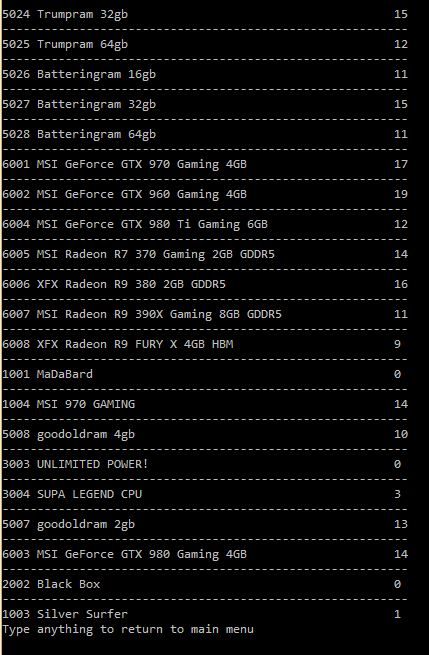
\includegraphics[scale=1]{Test1.jpg}
	\caption{The stock-list. Takes no input and thus no possibility for error, database excluded}
\end{figure}

\begin{figure}[H]\center
	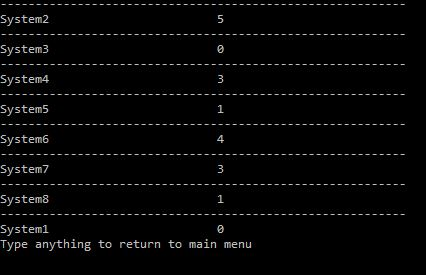
\includegraphics[scale=1]{Test2Systems.jpg}
	\caption{Systems that can be build. Not prone to error.}
\end{figure}

\begin{figure}[H]\center
	\includegraphics[scale=1]{Pricelisttest3.jpg}
	\caption{The price-list.}
\end{figure}

\begin{figure}[H]\center
	\includegraphics[scale=1]{Priceoffertest4.jpg}
	\caption{A price-offer for System1. It is possible throw an exception by inputting an incorrect name}
\end{figure}

\begin{figure}[H]\center
	\includegraphics[scale=1]{Saletest5.jpg}
	\caption{An example of a sale being inputted. Again, it is possible to throw an exception with incorrect input.}
\end{figure}

\begin{figure}[H]\center
	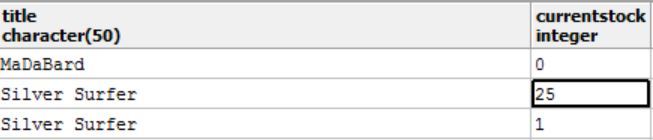
\includegraphics[scale=1]{10021.jpg}
	\caption{The database before a sale is inputted, for reference.}
\end{figure}
\begin{figure}[H]\center
	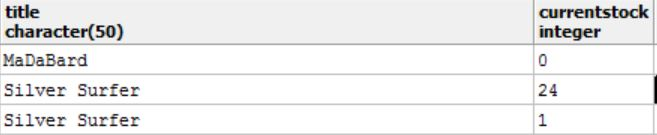
\includegraphics[scale=1]{10022.jpg}
	\caption{The database after a sale.}
\end{figure}

\begin{figure}[H]\center
	\includegraphics[scale=1]{test6restock.jpg}
	\caption{Restocking-list.}
\end{figure}

\begin{comment}
I testing skal i forklare jeres tests osv. udover det kan i have et billede med
som i kan tilføje ved at kopiere includegraphics som herunder.

\begin{figure}[H]\center
 \includegraphics[scale=1]{billede.png}
 \caption{}
\end{figure}

udskift billede.png med jeres billede fil som skal ligge i samme mappe som .tex
i kan ændre på scale for at ændre pÃ¥ billede størrelse i pdfen.
\end{comment}
\section{User-manual}

To best give an overview, the application is divided by the operations specified in the assignment. When initiating the program, the main menu will appear and the user can choose an operation by inputting the corresponding integer. Most of the operations will finish without further input, but 'price-offer' and 'execute sale' requires further input, the first by inputting one of the system-names and the second by inputting the kind of sale and name or modelnumber. Both of these are further described by the application, and ought to be fairly easy to navigate. 

\section{Conclusion} 

%hvad kom i frem til, gik noget galt? kunne noget gøres bedre?
Having finished the project and being able to look in retrospect, overall I am satisfied with the result. Some things, however, could have been better. During the project I preferred to keep error-handling in the java-application, for example the InStock-check operation, and together with this I did not implement actual constraints for creating a computersystem, making sure the parts matched. While these things are not required for the program to function properly, I do feel that in the spirit of this being a database-project, these things could have been implemented.

\newpage

\section{Appendix (source code)}
%lstinputlisting tilføjer jeres sourcecode, jeres python fil skal bare ligge i samme mappe som .tex filen husk at fjerne %

%\textbf{Sierpinski triangle program}
%\lstinputlisting[language=python]{sierpinski.py}
%\textbf{Binary tree program}
%\lstinputlisting[language=python]{binary.py}

\begin{figure}[H]\center
	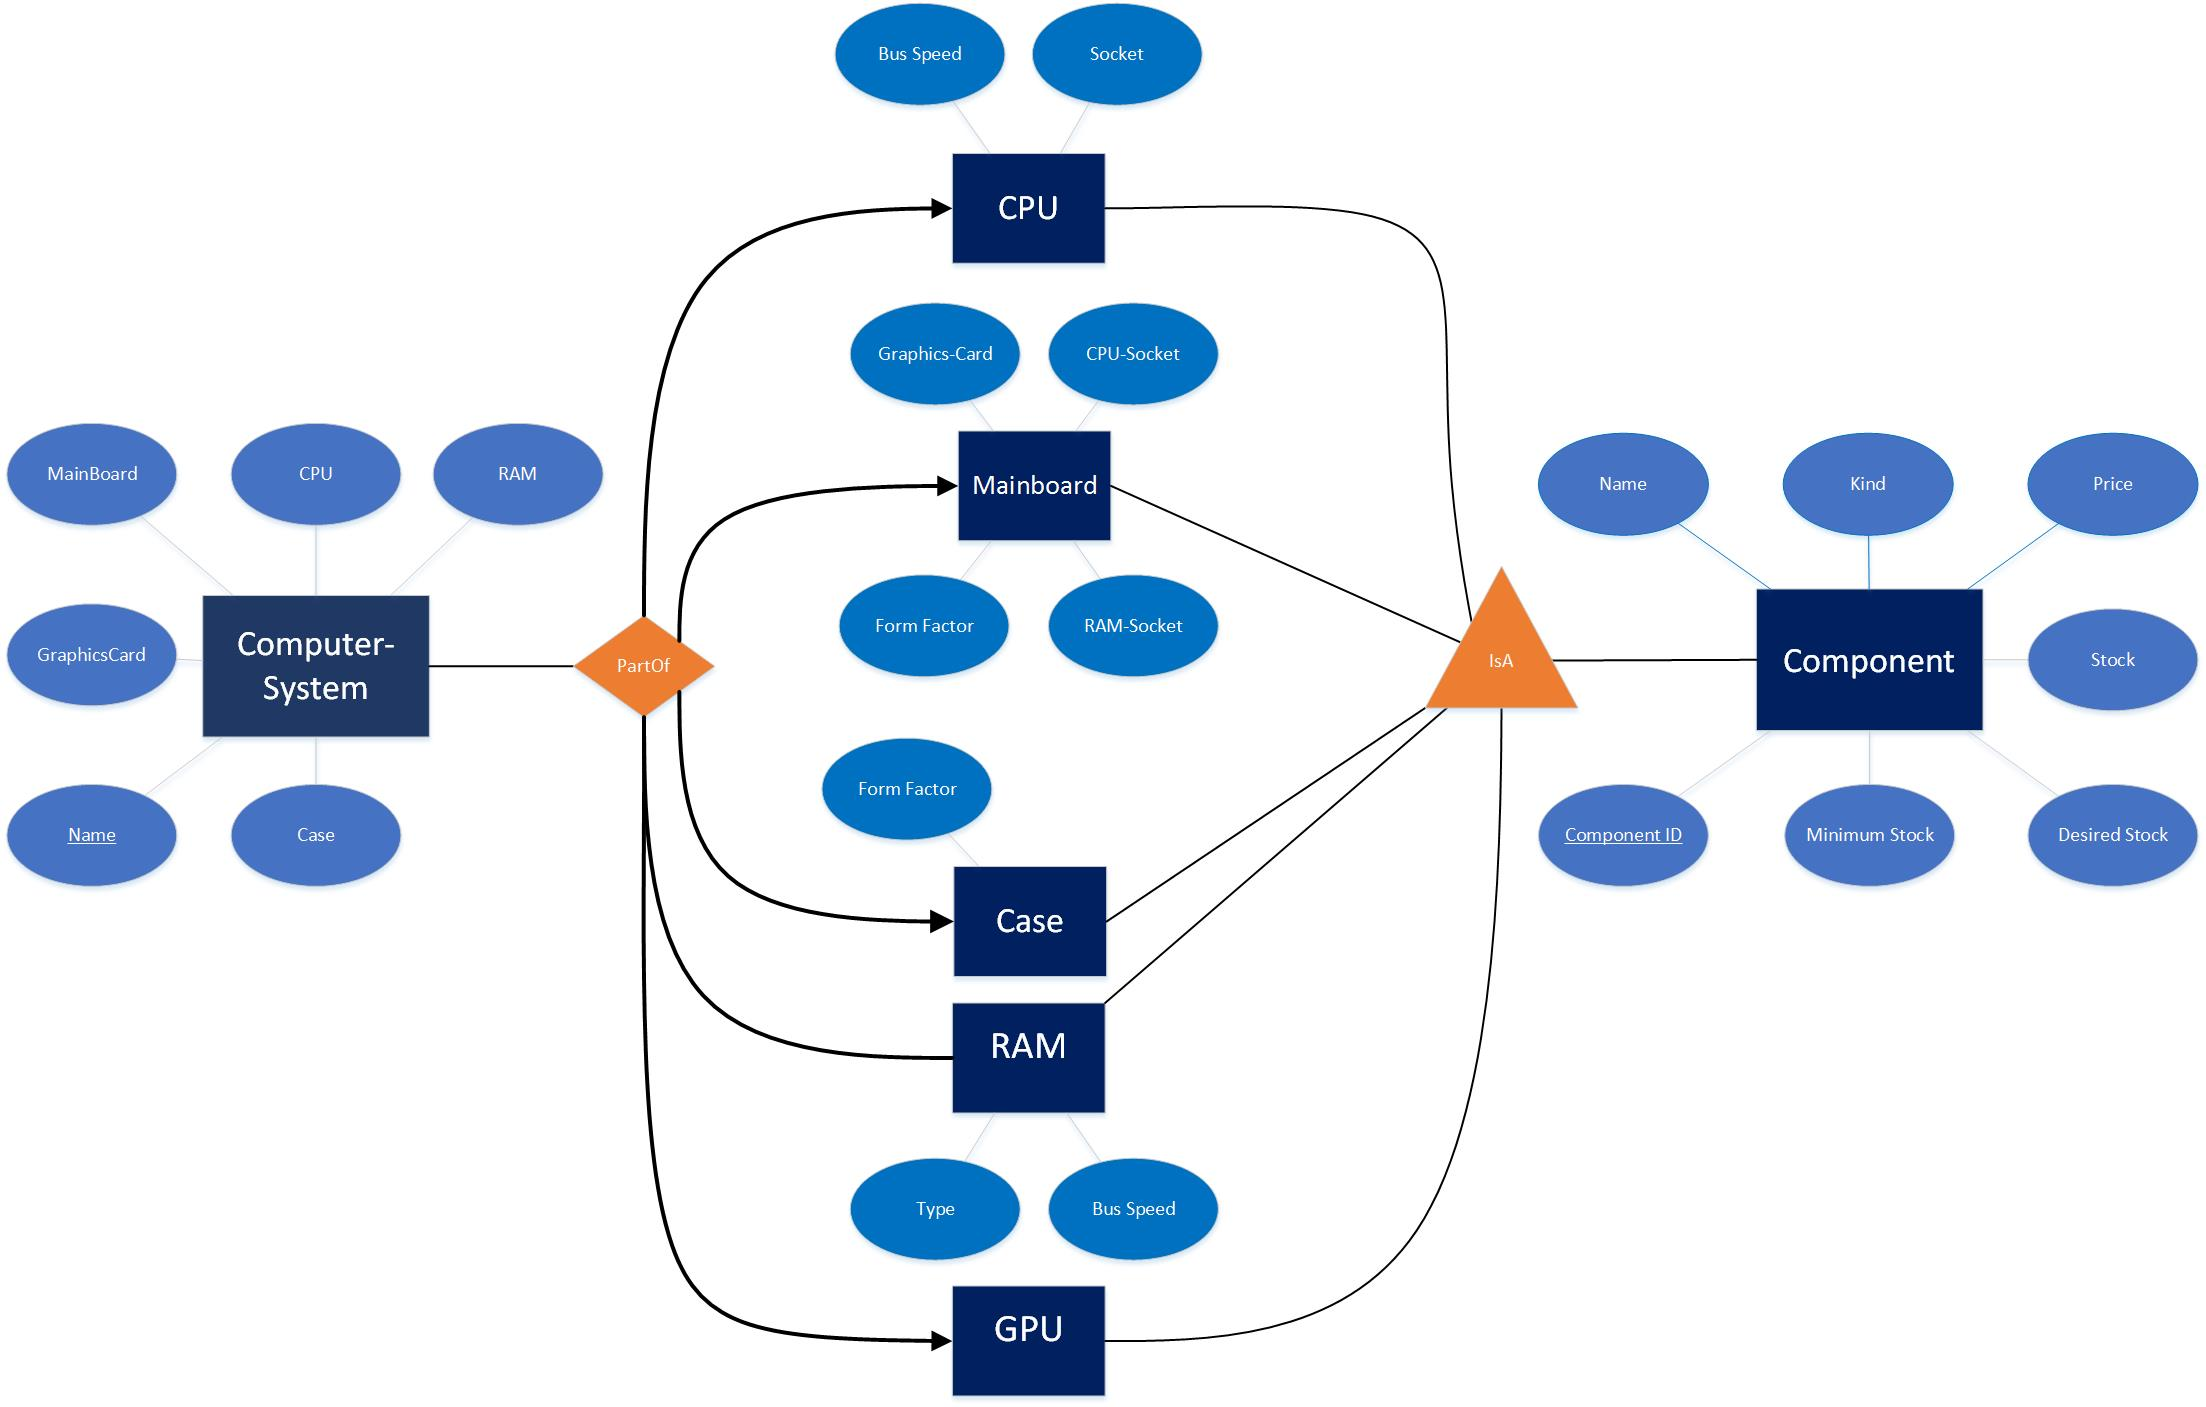
\includegraphics[scale=0.4]{E_R.jpg}
	\caption{The ER model for the database. Note some names are slightly different from the actual database, as this was created before beginning the programming (eg. component id = modelno).}
\end{figure}

\subsection{Relational model and arguments for 3nf}
Component(\underline{modelno},title,price,minimumstock,currentstock,preferredstock,kind)\\
CPU(\underline{modelno},busspeed,socket)\\
Mainboard(\underline{modelno},Graphicscard,CPU-socket,Form-factor,Ram-socket)\\
Case(\underline{modelno},Form-factor)\\
Ram(\underline{modelno},type,busspeed)\\
GPU(\underline{modelno})\\
Because the primary keys employed, 'modelno' and 'name' are the only ones upon which other data is dependent i.e no transitive dependencies, the data is in third normal. In other words, one can only extract a row from the tables by the modelno or in the case of 'Computer-system', by name. By adding the modelno, a unique identifier for all parts, this is possible.
\begin{comment}
Hvis Fern Time er lavet tilføjes det her og begin og end comment skal fjernes. 
\textbf{Fern program}
\lstinputlisting[language=python]{fern.py}
\end{comment}
Note I include the source code for the java-application in this pdf. The SQL-piece can be found in the .query file included as well as the database dump.
\lstinputlisting[language=java]{test.java}


\end{document}
